\chapter{sounds}
\lhead[tempest 2000]{}
\label{sec:listing}
\lstset{style=68KStyle}

The sound effects in Tempest 2000 are stpred in the game as Pulse Code Modulation (PCM) data. This is the most common format for storing
raw audio and flavors of it are used in everything from CDs to telephony. PCM data is as simple as a stream of numbers. Each of the numbers
is between a lower and upper limit:, for example between -128 and 128. If you plot enough of these numbers along a graph you get what looks like
a wave. This is pretty much the sound wave, the analog version of our digital values. If you put these values through the right piece of hardware,
such as a Digital Analog Converter (DAC) you can get a sound out the other side.

\begin{figure}[H]
    \centering
    \begin{adjustbox}{width=7cm,center}
      \frame{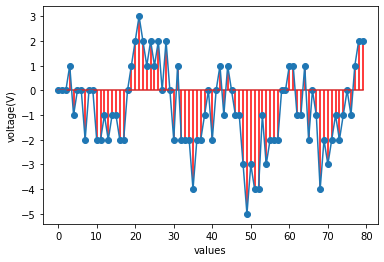
\includegraphics[width=4cm]{src/sounds/sample.png}}%
    \end{adjustbox}
  \caption{A sample of 80 bytes plotted as a wave graph.}
\end{figure}

The PCM data in Tempest 2000's sound samples is nothing more than this series of bytes, each one representing a value between -128 and 128, which can
be converted into sound. A single series of bytes will give us one 'channel' of sound, i.e. a mono sound sample. What we actually have are stereo
sound samples so each sample contains two channels. The simplest way of incorporating two separate channels in the sample (one for the left speaker
and one for the right) is to interleave them, in alternating bytes. We can see that this is the way the Tempest samples are encoded if we split out
an arbitrary sample into separate streams of alternate bytes and graph them.

\begin{figure}[H]
    \centering
    \begin{adjustbox}{width=12cm,center}
      \frame{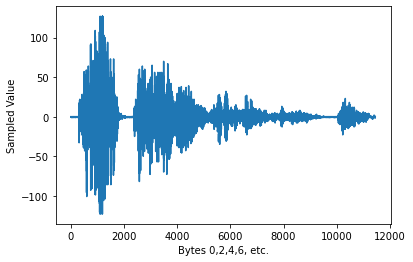
\includegraphics[width=4cm]{src/sounds/samplel.png}}%
      \hspace{0.5cm}
      \frame{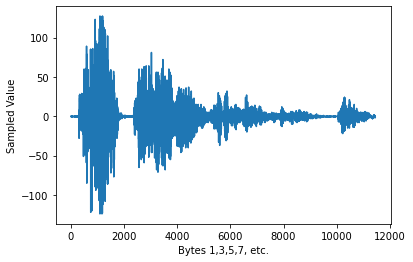
\includegraphics[width=4cm]{src/sounds/sampler.png}}%
    \end{adjustbox}
  \caption{Plotted sound waves for the left and right channels respectively.}
\end{figure}

Since the sounds we want to play are just blobs of data, we need a way of knowing where these blobs are, and perhaps
some information on what we have to do with them. This is provided by \icode{samtab}, a block of data at address
\icode{\$9ac800} that tells us everything we need to know:

\begin{lstlisting}
  samtab       EQU $9ac800
\end{lstlisting}

Just byt itself, the \icode{samtab} table reveals some interesting potential for ways that we can use the
raw PCM bytes. 

\begin{lstlisting}[basicstyle=\scriptsize\ttfamily,caption=The contents of \icode{samtab} at \icode{\$9AC800}.]
;                       Prio-                                  Repeat     Repeat
;Name                   rity   Period Start      Length        Start      Length      
;---------------------- -----  ------ ---------  -------  --   ---------  -------  ---
'Engine Noise 1      ', $0001, $01ac, $009acd00, $0011a0, $00, $009acd02, $00119e, $00
'Player Shot Normal 2', $0002, $01ac, $009adea4, $0008e8, $00, $009adea4, $000000, $00
'Engine Noise        ', $0003, $01ac, $009ae290, $003378, $00, $009aee9e, $002594, $00
'Player Death        ', $0004, $00d6, $00000000, $00549a, $00, $00000000, $000000, $00
'Player Death 2      ', $0005, $01ac, $00000000, $002458, $00, $00000000, $000000, $00
'Player Shot Normal  ', $0006, $01ac, $009b160c, $0007a4, $00, $009b160c, $000000, $00
'Player Jump         ', $0007, $01ac, $009b1db4, $0018de, $00, $009b1db4, $000000, $00
'Crackle             ', $0008, $00d6, $009b3696, $004594, $00, $009b3696, $000000, $00
'Cleared Level       ', $0009, $01ac, $009b7c2e, $0037a2, $00, $009b7c2e, $000000, $00
'Warp                ', $000a, $0238, $009bb3d4, $006ec8, $00, $009bb3d4, $000000, $00
'Large Explosion     ', $000b, $01ac, $009c22a0, $0050c2, $00, $009c22a0, $000000, $00
'Powered Up Shot     ', $000c, $01ac, $009c7366, $001976, $00, $009c7366, $000000, $00
'Get Power Up        ', $000d, $01ac, $009c8ce0, $001aea, $00, $009c8ce0, $000000, $00
'Tink For Spike      ', $000e, $00fe, $009ca7ce, $00040e, $00, $009ca7ce, $000000, $00
'NME At Top Of Web   ', $000f, $01ac, $009cabe0, $00001e, $00, $009cabe0, $000000, $00
'Pulse For Pulsar    ', $0010, $0358, $009cac02, $0019fe, $00, $009cac02, $000000, $00
'Normal Explosion    ', $0011, $00d6, $009cc604, $002ab6, $00, $009cc604, $000000, $00
'Extra Explosion     ', $0012, $0358, $009cf0be, $0018ca, $00, $009cf0be, $000000, $00
'Static or Pulsar    ', $0013, $011c, $009d098c, $003fe4, $00, $009d098c, $000000, $00
'Pulsar Pulse        ', $0014, $0358, $009d4974, $000f0c, $00, $009d4974, $000000, $00
'Off Shielded NME    ', $0015, $00aa, $009d5884, $0027ca, $00, $009d5884, $000000, $00
'Excellent           ', $0016, $0200, $009d8052, $005976, $00, $009d8052, $000000, $00
'Superzapper Recharge', $0016, $0200, $009dd9cc, $00a958, $00, $009dd9cc, $000000, $00
'yes                 ', $0018, $0200, $009e8328, $005a6c, $00, $009e832a, $005a6a, $00
'oneup               ', $0019, $0200, $009edd98, $0043ae, $00, $009edd98, $000000, $00
'screeeam            ', $001a, $0200, $009f214a, $004568, $00, $009f214a, $000000, $00
'sexy yes 1          ', $001b, $0200, $009f66b6, $002c54, $00, $009f66b6, $000000, $00
'sexy yes 2          ', $001c, $0200, $009f9362, $003236, $00, $009f9362, $000000, $00
'tink                ', $001e, $0200, $009fc59c, $0005ce, $00, $009fc59c, $000000, $00
'zero                ', $001f, $0200, $009fcb6e, $000008, $00, $009fcb6e, $000000, $00
'dummy               ', $0020, $0200, $009fcb7a, $00a1d8, $00, $009fcb7a, $000000, $00
\end{lstlisting}

Of course the best way of seeing how this works is to follow one through in practice. Here
is the little routine that shouts 'Excellent!' when you navigate the options menu. We can
see that we do a little set up such as selecting the sample from the table above ('Excellent'
is at position 21 (\icode{\$16} in hex)), setting its pitch and then calling another routine
called \icode{fox} that inches nearer the actual work of playing the sample:

\begin{lstlisting}
; *******************************************************************
; Say 'Excellent', e.g. when the user naviates to an option.
; *******************************************************************
sayex:
  move #21,sfx           ; Select effect $16 (21) from samtab, 'Excellent'.
  move #101,sfx_pri      ; Set the priority.
  ;move #$ff,sfx_vol     ; Setting the volume is commented out.
  move.l #$160,sfx_pitch ; Set the pitch.
  jsr fox                ; Play the effect (see below).
  move #101,sfx_pri      ; Do it again.
  ;move #$ff,sfx_vol
  move.l #$162,sfx_pitch ; This time with a different pitch.
  jmp fox                ; Play it.
\end{lstlisting}

\icode{fox} (why waste an opportunity to pun on  something in the animal kingdom) sets
up our data for playing the sample. It's main preoccupation is turning our index into
the \icode{samtab} table to a pointer to the data there.

\begin{lstlisting}
; *******************************************************************
; Play a selected sound sample.
; *******************************************************************
fox:
  movem.l d0-d3/a0,-(a7)  ; Save d0,d1,d2,d3,a0 to the a7 register.
                          ; Because we're going to clobber them here.
  move sfx,d0             ; Store sfx in d0, this is '$16' for 'Excellent'.

  ; Use '21' to point to the address of sample data, i.e. directly after
  ; the 'Excellent    ' in this entry in samtab:
  ; 'Excellent           ', $0016, $0200, $009d8052, $005976, $00, 

  ; Since each entry in samtab is 40 bytes long, multiplying our index by
  ; 40 will bring us to the start of the 'Excellent' entry. The steps below
  ; are a fast way of doing this multiplication by 40.
  lsl #3,d0   ; Turn $16(21) into $a8 by left-shifting. 
  move d0,d1  ; Store in d1.
  lsl #2,d0   ; Turn $a8 into $2a0 by left-shifting.           
  add d1,d0   ; d0 is now $348 (840), i.e. 21 * 40. 

  ; Now that we have an offset for our sample information in samtab, we'll
  ; add 20 to it (so that it's after the sample name) and store it in a0.
  lea samtab,a0           ; Store samtab address in a0.
  lea 20(a0,d0.w),a0      ; Add 840 + 20 to it. 

  ; Now we can set up the last few items our sound synth needs.
  move sfx_pri,d1
  move sfx_vol,d2
  move.l sfx_pitch,d3

  ; Invoke the sound synth to play our sample.
  jsr PLAYFX2

  ; Clean up.
  move d0,handl
  clr sfx_pri
  clr sfx_vol
  clr.l sfx_pitch

  movem.l (a7)+,d0-d3/a0 ; Restore the old unclobbered values we saved off
                         ; at the start.
  rts
\end{lstlisting}

To recap, at this point we have set up our registers as follows:

\begin{figure}[H]
  {
    \setlength{\tabcolsep}{3.0pt}
    \setlength\cmidrulewidth{\heavyrulewidth} % Make cmidrule = 
    \begin{adjustbox}{width=10cm,center}

      \begin{tabular}{lll}
        \toprule
        Register & Value & Description\\
        \midrule
        \icode{a0} & \icode{\$9acb5c} & Address of the 'Excellent' metadata in \icode{samtab}. \\
        \icode{d1} & \icode{101} & \icode{sfx\_pri}. \\
        \icode{d2} & \icode{\$ff} & \icode{sfx\_vol}: the volume to play at. \\
        \icode{d3} & \icode{\$162} & \icode{sfx\_pitch}: the pitch to play at. \\
        \bottomrule
      \end{tabular}
    \end{adjustbox}
  }
\end{figure}

These are the garnish for a choice piece of mystery meat, \icode{PLAYFX2}. \icode{PLAYFX2} is a
library routine provided to Atari by a crowd called 'Imagitec Designs'. It is not something we have the source
code for, and nor did Minter when he was writing Tempest 2000. Instead, he was given a binary blob
called \icode{syn6.o} and a list of routine names to use when he wanted to play one of his samples.
This list is given at the start of the main \icode{yak.s} source file:

\begin{lstlisting}
  INIT_SOUND    EQU  $4040  ;jump table for the SFX/Tunes module
  NT_VBL        EQU  $4046
  PT_MOD_INIT   EQU  $404c
  START_MOD     EQU  $4052
  STOP_MOD      EQU  $4058
  PLAYFX2       EQU  $405e
  CHANGE_VOLUME EQU  $4064
  SET_VOLUME    EQU  $406a
  NOFADE        EQU  $4070
  FADEUP        EQU  $4076
  FADEDOWN      EQU  $407c
  ENABLE_FX     EQU  $4082
  DISABLE_FX    EQU  $4088
  CHANGEFX      EQU  $409a  ;new in syn6
  HALT_DSP      EQU  $408e
  RESUME_DSP    EQU  $4094
  intmask       EQU  $40a0
\end{lstlisting}

These are all entry points in the game binary for each routine. So for \icode{PLAYFX2} the entry point is \icode{\$405e}.
In the source code this routine exists as raw machine code only. Along with all the other Imagitec sound routines it
lives in a file called \icode{moomoo.dat}:
\begin{lstlisting}
  .include "moomoo.dat"
\end{lstlisting}

This is a slightly modified version of the \icode{syn6.o} sound synthesizer binary provided by Imagitec Designs. With modern
tooling, it is possible for us to recreate \icode{moomoo.dat} by partially disassembling it, then reassembling and relinking it.
This will more or less re-enact the build steps Minter would have followed to generate it.

The initial bytes of \icode{moomoo.dat} can be disassembled as follows into a file we'll call \icode{moomoo\_header.s}. 
\begin{lstlisting}[caption=The contents of \icode{moomoo\_header.s}.]
; Header for moomoo.s
;.org $4040
.include "jaguar.inc"

init_sound    EQU $000041ba
nt_vbl        EQU $0000425e
pt_mod_init   EQU $000041d6
start_mod     EQU $000045e2
stop_mod      EQU $00004606
playfx2       EQU $00004370
change_volume EQU $000044ea
set_volume    EQU $00004546
nofade        EQU $00004598
fadeup        EQU $000045b2
fadedown      EQU $000045ca
enable_fx     EQU $0000464e
disable_fx    EQU $00004660
resume_dsp    EQU $00004470

INIT_SOUND:    jmp     (init_sound).l
NT_VBL:        jmp     (nt_vbl).l
PT_MOD_INIT:   jmp     (pt_mod_init).l
START_MOD:     jmp     (start_mod).l
STOP_MOD:      jmp     (stop_mod).l
PLAYFX2:       jmp     (playfx2).l
CHANGE_VOLUME: jmp     (change_volume).l
SET_VOLUME:    jmp     (set_volume).l
NOFADE:        jmp     (nofade).l
FADEUP:        jmp     (fadeup).l
FADEDOWN:      jmp     (fadedown).l
ENABLE_FX:     jmp     (enable_fx).l
DISABLE_FX:    jmp     (disable_fx).l
CHANGEFX:      jmp     (disable_fx).l
HALT_DSP:      jmp     (disable_fx).l
RESUME_DSP:    jmp     (resume_dsp).l

intmask:        dc.b 0
; Address 0x40A2
return_early:
                rts

; Address 0x40A4
update_interrupt:
                move.w  d0,-(sp)
                bset    #3,(intmask).l
                clr.w   d0
                move.b  (intmask).l,d0
                move.w  d0,(INT1).l ; RW CPU Interrupt Control Register
                move.w  (sp)+,d0
                rts
\end{lstlisting}

It turns out that the address we're using to invoke \icode{PLAYFX2} simply jumps to another adress in the binary,
one that contains the actual \icode{playfx2} routine:

\begin{lstlisting}
PLAYFX2:       jmp     (playfx2).l
\end{lstlisting}

So to recreate the steps used to generate \icode{moomoo.dat} we first assemble this file:

\begin{lstlisting}
rmac -fa -i moomoo_header.s -o moomoo_header.o
\end{lstlisting}

Then we link \icode{moomoo\_header.o} with the \icode{syn6.o} file provided by Imagitec:
\begin{lstlisting}
rln -n -z -u -v -a 4040 xd xd -e moomoo_header.o syn6.o -o moomoo.dat
\end{lstlisting}

Voila, we have our \icode{moomoo.dat}. If you'd like to follow these steps yourself, \href{https://github.com/mwenge/t2k-25easypieces/blob/master/notebooks/Recreate%20moo.dat/Recreate%20moomoo.dat%20using%20syn6.o.ipynb}{\textcolor{blue}{you can use this Python notebook}}.

\begin{figure}[H]
{
\setlength{\tabcolsep}{1.0pt}
\setlength\cmidrulewidth{\heavyrulewidth} % Make cmidrule = 
\begin{adjustbox}{width=14cm,center}
\begin{tabular}{ccc}
\toprule
Spectrogram & Amplitude & Sound \\
\midrule
  \makecell[l]{
    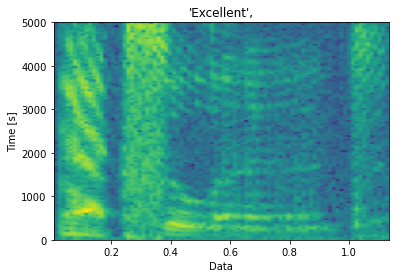
\includegraphics[width=6cm]{sounds/22.wav-spec.png}%
  } &
  \makecell[l]{
    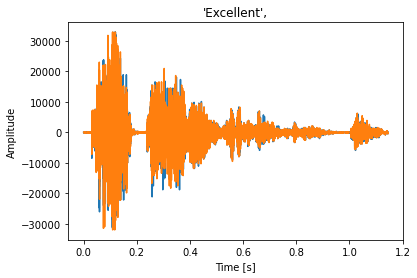
\includegraphics[width=6cm]{sounds/22.wav-amp.png}%
  } &
  \makecell[l]{
    \textattachfile{src/sounds/22.wav}{
\includegraphics[width=1cm]{sounds/play.png}}
  } \\
  \addlinespace
    \bottomrule
    \end{tabular}
  \end{adjustbox}
}\caption{Spectrogram and Sine Plot of the 'Excellent' sound sample. On a PDF viewer that supports, it you can click 'Play' to hear it.}
\end{figure}
